\subsection{External Interface Requirements}
\subsubsection{User Interfaces}
\hspace{\parindent}The CLup application interface will have to serve two types of users: customers and store managers. Opening screen of the application allows the user to pick a store or to login as a store manager. Depending on the choice, another screen is presented. For a customer, a screen with the options to retrieve a ticket, book a visit or change the store. For a store manager, a screen containing their camera view, and buttons to confirm the scanned ticket, notify the system about a customer exit and to log out of the application. 

The following images show some basic concepts on how the app should look on both Android and iOS devices.
\captionsetup{justification=centering}

\begin{figure}[!htb]
\centering
\begin{minipage}{0.4\textwidth}
\centering

\includegraphics[width=0.8\textwidth]{Images/App/Logov2_Blue2_Bck}
\caption{\label{fig:android1}\textbf{Logo concept}}
\end{minipage}
\begin{minipage}{0.4\textwidth}
\centering

\includegraphics[width=0.3\textwidth]{Images/App/AppIcon}
\captionsetup{justification=centering}
\caption{\label{fig:ios1}\textbf{App icon concept}}
\end{minipage}
\end{figure}

\begin{figure}[!htb]
\centering
\begin{minipage}{0.4\textwidth}
\centering
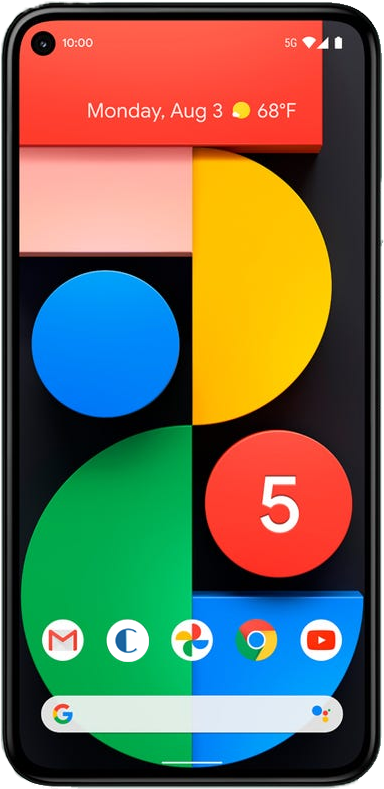
\includegraphics[width=0.8\textwidth]{Images/App/Android_AppIcon}
\caption{\label{fig:android1}\textbf{Android app 1}}
\end{minipage}
\begin{minipage}{0.4\textwidth}
\centering
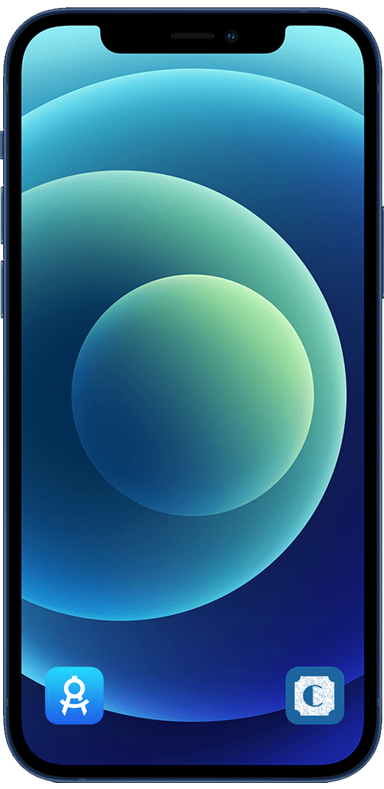
\includegraphics[width=0.8\textwidth]{Images/App/iPhone_AppIcon}
\captionsetup{justification=centering}
\caption{\label{fig:ios1}\textbf{iOS app 1}}
\end{minipage}
\end{figure}

\newpage

\begin{figure}[!h]
\centering
\begin{minipage}{0.4\textwidth}
\centering
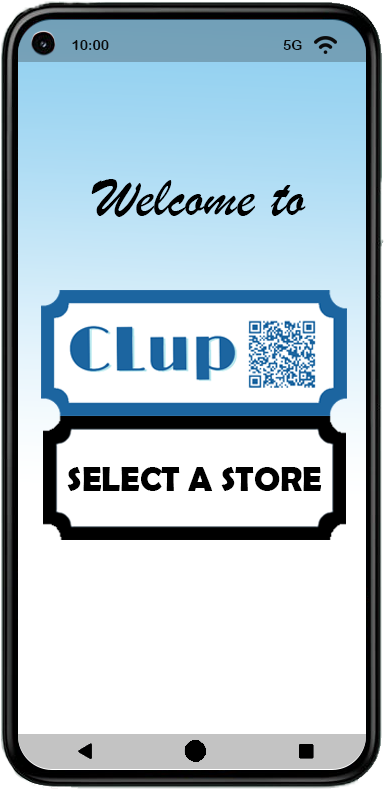
\includegraphics[width=0.75\textwidth]{Images/App/Android_HomeScreenv2}
\caption{\label{fig:android2}\textbf{Android app 2}}
\end{minipage}
\begin{minipage}{0.4\textwidth}
\centering
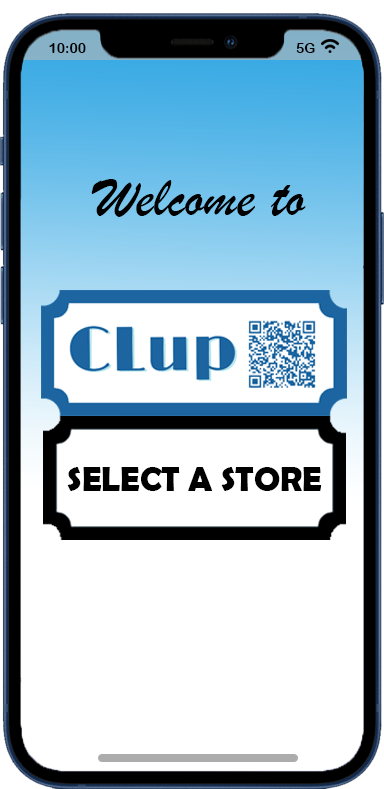
\includegraphics[width=0.75\textwidth]{Images/App/iPhone_HomeScreenv2}
\captionsetup{justification=centering}
\caption{\label{fig:ios2}\textbf{iOS app 2}}
\end{minipage}
\end{figure}

\begin{figure}[!b]
\centering
\begin{minipage}{0.4\textwidth}
\centering
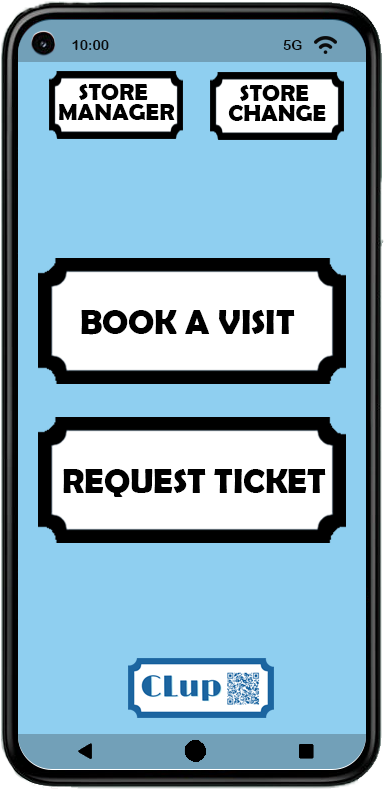
\includegraphics[width=0.75\textwidth]{Images/App/Android_MainScreenv2}
\caption{\label{fig:android3}\textbf{Android app 3}}
\end{minipage}
\begin{minipage}{0.4\textwidth}
\centering
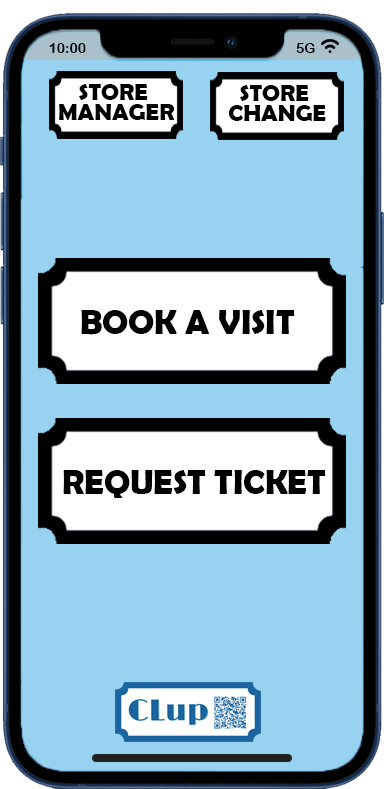
\includegraphics[width=0.75\textwidth]{Images/App/iPhone_MainScreenv2}
\captionsetup{justification=centering}
\caption{\label{fig:ios3}\textbf{iOS app 3}}
\end{minipage}
\end{figure}

\begin{figure}[!h]
\centering
\begin{minipage}{0.4\textwidth}
\centering
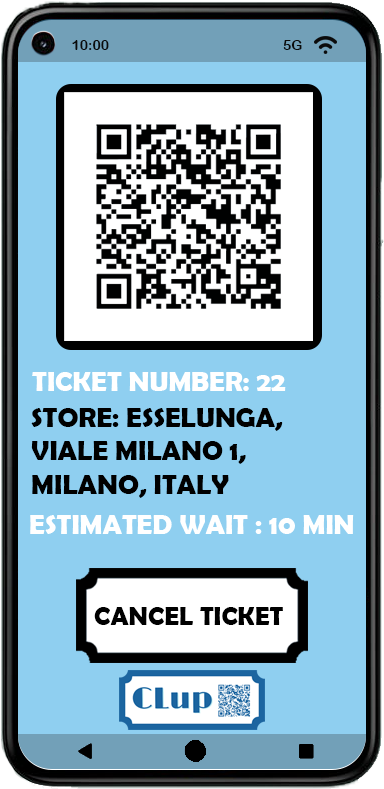
\includegraphics[width=0.75\textwidth]{Images/App/Android_RequestTicket}
\caption{\label{fig:android3}\textbf{Android app 3}}
\end{minipage}
\begin{minipage}{0.4\textwidth}
\centering
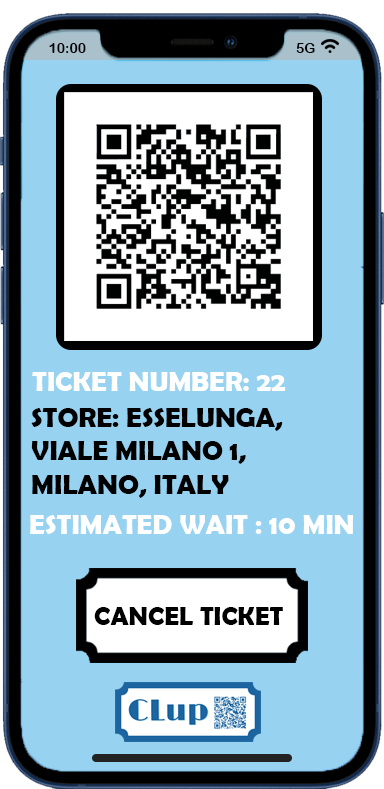
\includegraphics[width=0.75\textwidth]{Images/App/iPhone_RequestTicket}
\captionsetup{justification=centering}
\caption{\label{fig:ios3}\textbf{iOS app 3}}
\end{minipage}
\end{figure}

\newpage

\subsubsection{Hardware Interfaces}
\hspace{\parindent}Depending on the current user the CLup application will require access to some hardware interfaces. If the current user is a customer, the application will require the device's camera and if the current user is the store manager the GPS location data will be needed. The application will require no further hardware interfaces.
\subsubsection{Software Interfaces}
\hspace{\parindent}The CLup application will not require any specific software interfaces.
\subsubsection{Communication Interfaces}
\hspace{\parindent}The most important communication will occur between the device and the database. The decision on the specific communication interface which will be used depends on the database, and is, therefore, left to the developers.

\newpage
\subsection{Functional Requirements}

\begin{enumerate}
			\item [\textbf{R1}] The user must be able to select a specific store in which they want to do the shopping.
			\item [\textbf{R2}] The user must be able to request a number and a ticket.
			\item [\textbf{R3}] The user must be able to receive a number and a ticket.
			\item [\textbf{R4}] The user must be able to physically retrieve a ticket from the printer containing a number and a QR code.
			\item [\textbf{R5}] A new ticket must be printed whenever a user physically retrieves the old one.
			\item [\textbf{R6}] The store manager must be able to scan a QR code.
			\item [\textbf{R7}] The store manager must be informed by the application if a user tries to enter the store out of order.
			\item [\textbf{R8}] The store manager must be informed when the capacity of the store is full.
			\item [\textbf{R9}] The store manager must be able to alert the system whenever a customer exits the store.
			\item [\textbf{R10}] The store manager must be provided with the login credentials upon request to the system administrator.	
			\item [\textbf{R11}] Allow the user to receive a precise estimation of waiting time when retrieving a number.
			\item [\textbf{R12}] The system must calculate an estimation of the waiting time based on data.
			\item [\textbf{R13}] The system must be able to update its estimated waiting time in real time.
			\item [\textbf{R14}] The system must be able to send an update to the user in specific intervals regarding estimated waiting time until it's their turn.
			\item [\textbf{R15}] The user must be able to request to see all the available timeslots in that specific store.
			\item [\textbf{R16}] The system must be able to provide the user with the list of all available timeslots upon the request.
			\item [\textbf{R17}] The user must be able to select a specific timeslot.
			\item [\textbf{R18}] The user must be able to receive a confirmation of his timeslot reservation, along with a number and a ticket.
			\item [\textbf{R19}] Allow the user to be at most five minutes late for his reservation before cancelling his ticket.
			\item [\textbf{R20}] The user must be able to specify expected duration of his visit to the store.
			\end{enumerate}			
\newpage
		
\subsubsection{Mapping}	

\begin{enumerate}
	\item [\textbf{G1}] Allow the user to "line up"/retrieve a number.
	\begin{enumerate}
		\item [\textbf{G1.1}] Allow the user to retrieve a number through the application.
		\begin{enumerate}
			\item [\textbf{R1}] The user must be able to select a specific store in which they want to do the shopping.
			\item [\textbf{R2}] The user must be able to request a number and a ticket.
			\item [\textbf{R3}] The user must be able to receive a number and a ticket.
			\item [\textbf{D4}] The registered store is a physical store, not a virtual store.
			\item [\textbf{D8}] The system can correctly save data about enter and exit times of anonymous customers to calculate estimated waiting time.
			\item [\textbf{D11}] The user has internet connection for the device at all times.
		\end{enumerate}
		\item [\textbf{G1.2}] Allow the user to retrieve a number physically from the printer.
		\begin{enumerate}
			\item [\textbf{R4}] The user must be able to physically retrieve a ticket from the printer containing a number and a QR code.
			\item [\textbf{R5}] A new ticket must be printed whenever a user physically retrieves the old one.	
			\item [\textbf{D8}] The system can correctly save data about enter and exit times of anonymous customers to calculate estimated waiting time.	
		\end{enumerate}
	\end{enumerate}
	\item [\textbf{G2}] Allow the store manager to control the entrance of customers via QR code scanning.
	\begin{enumerate}
		\item [\textbf{R6}] The store manager must be able to scan a QR code.
		\item [\textbf{R7}] The store manager must be informed by the application if a user tries to enter the store out of order.
		\item [\textbf{R8}] The store manager must be informed when the capacity of the store is full.
		\item [\textbf{R9}] The store manager must be able to alert the system whenever a customer exits the store.
		\item [\textbf{R10}] The store manager must be provided with the login credentials upon request to the system administrator.
		\item [\textbf{D1}] The store manager's username must be unique. 
		\item [\textbf{D2}] The store manager can observe both entering and exiting customers.
		\item [\textbf{D3}] The store manager's password must be secure. 
		\item [\textbf{D5}] The screen of the user's phone is scannable and not to damaged.
		\item [\textbf{D8}] The system can correctly save data about enter and exit times of anonymous customers to calculate estimated waiting time.
		\item [\textbf{D11}] The user has internet connection for the device at all times.


	\end{enumerate}
	\item [\textbf{G3}] Allow the user to get precise calculations of the waiting time.
	\begin{enumerate}
		\item [\textbf{R11}] Allow the user to receive a precise estimation of waiting time when retrieving a number.
		\item [\textbf{R12}] The system must calculate an estimation of the waiting time based on data.
		\item [\textbf{D4}] The registered store is a physical store, not a virtual store.
		\item [\textbf{D7}] The system can use data about the user to calculate estimated waiting time.
		\item [\textbf{D8}] The system can correctly save data about enter and exit times of anonymous customers to calculate estimated waiting time.
		\item [\textbf{D11}] The user has internet connection for the device at all times.
	\end{enumerate}
	\item [\textbf{G4}] Allow the user to be updated on the store waiting time situation.
	\begin{enumerate}
		\item [\textbf{R13}] The system must be able to update its estimated waiting time in real time.
		\item [\textbf{R14}] The system must be able to send an update to the user in specific intervals regarding estimated waiting time until it's their turn.
		\item [\textbf{D4}] The registered store is a physical store, not a virtual store.
		\item [\textbf{D7}] The system can use data about the user to calculate estimated waiting time.
		\item [\textbf{D8}] The system can correctly save data about enter and exit times of anonymous customers to calculate estimated waiting time.
		\item [\textbf{D11}] The user has internet connection for the device at all times.
	\end{enumerate}
	\item [\textbf{G5}] Allow the user to "Book a visit" to the store.
	\begin{enumerate}
			\item [\textbf{R15}] The user must be able to request to see all the available timeslots in that specific store.
			\item [\textbf{R16}] The system must be able to provide the user with the list of all available timeslots upon the request.
			\item [\textbf{R17}] The user must be able to select a specific timeslot.
			\item [\textbf{R18}] The user must be able to receive a confirmation of his timeslot reservation, along with a number and a ticket.
			\item [\textbf{R19}] Allow the user to be at most five minutes late for his reservation before cancelling his ticket.
			\item [\textbf{R20}] The user must be able to specify expected duration of his visit to the store.
			\item [\textbf{D4}] The registered store is a physical store, not a virtual store.
			\item [\textbf{D6}] The user's device provides accurate GPS information.
			\item [\textbf{D7}] The system can use data about the user to calculate estimated waiting time.
			\item [\textbf{D8}] The system can correctly save data about enter and exit times of anonymous customers to calculate estimated waiting time.
			\item [\textbf{D9}] The system can correctly save and pull data from available timeslot tables in the database.
			\item [\textbf{D10}] The system can update timeslot tables at any moment while available.
			\item [\textbf{D11}] The user has internet connection for the device at all times.
	\end{enumerate}
\end{enumerate}

\newpage
\begin{table}[!htb]
\centering
\begin{tabular}{|
>{\columncolor[HTML]{EFEFEF}}l |l|l|}
\hline
\cellcolor[HTML]{C0C0C0}\textbf{Goal, {[}Gn{]}} & \cellcolor[HTML]{C0C0C0}\textbf{Requirements, {[}Rn{]}} & \cellcolor[HTML]{C0C0C0}\textbf{Domains, {[}Dn{]}} \\ \hline
 &   & \\
G1.1 & R1, R2, R3, R4 & D4, D8, D11         \\ 
&   & \\ \hline
&   & \\
G1.2  & R4, R5 & D8         \\ 
&   & \\ \hline
&   & \\
G2  & R6, R7, R8, R9, R10 & D1, D2, D3, D5, D8, D11         \\
&   & \\ \hline
&   & \\
G3  & R11, R12 & D4, D7, D8, D11         \\ 
&   & \\ \hline
&   & \\
G4  & R13, R14 & D4, D7, D8, D11     \\ 
&   & \\ \hline
&   & \\
G5  & R15, R16, R17, R18, R19, R20 & D4, D6, D7, D8, D9, D10, D11    
 \\
&   & \\ \hline
\end{tabular}
\caption{\textbf{Mapping table}}
\label{tab:my-table}
\end{table}
\newpage

\subsubsection{Use cases}

\begin{table}[H]
\centering
\begin{tabular}{|
>{\columncolor[HTML]{EFEFEF}}l |l|}
\hline
Name                 & \textbf{Book a visit}                                                                                               \\ \hline
Actors               & \textbf{User}                                                                                                       \\ \hline
Goals                & \textbf{G5}                                                                                                         \\ \hline
Entry condition      & \begin{tabular}[c]{@{}l@{}}User has the application installed \\ Desired store is in the CLup database\end{tabular} \\ \hline
Event flow &
  \begin{tabular}[c]{@{}l@{}}User opens the CLup application \\ User selects a store \\ User selects "Book a visit" \\ System sends user a list of available timeslots \\ User selects a specific timeslot \\ User inputs the estimated shopping time (optional) \\ User enables location services (optional) \\ If user has enabled location services \\ System calculates distance to the store \\ User receives estimated traveling time to the store \\ User receives a number and a QR code\end{tabular} \\ \hline
Exit condition       & Ticket request is successful                                                                                        \\ \hline
Exception            & There are no available timeslots, user can search for a another store                                               \\ \hline
Special requirements & \textbf{/}                                                                                                          \\ \hline
UMLs                 & \textbf{\hyperref[fig:usecase1]{Use case}, \hyperref[fig:sequence4]{Sequence}, \hyperref[fig:statechart2]{State chart}}                                                             
\\ \hline
\end{tabular}
\caption{\textbf{Use case - Book a visit}}
\label{tab:my-table}
\end{table}

\begin{table}[H]
\centering
\begin{tabular}{|
>{\columncolor[HTML]{EFEFEF}}l |l|}
\hline
Name           & \textbf{Retrieve a number (in person)} \\ \hline
Actors         & \textbf{User, Store manager}           \\ \hline
Goals          & \textbf{G1.2}                            \\ \hline
Entry condition &
  \begin{tabular}[c]{@{}l@{}}User present at the store \\ Desired store is in the CLup database\end{tabular} \\ \hline
Event flow &
  \begin{tabular}[c]{@{}l@{}}User goes to the ticket machine and takes a ticket \\ User waits for his number \\ Store manager scans user's QR code \\ User enters the store\end{tabular} \\ \hline
Exit condition & User exits the store                   \\ \hline
Exception &
  \begin{tabular}[c]{@{}l@{}}The ticket printer is not working, user waits for it to be fixed \\ The QR code cannnot be scanned due to damaged ticket, \\ user gets another ticket\end{tabular} \\ \hline
Special requirements &
  \begin{tabular}[c]{@{}l@{}} A new ticket gets printed in less \\ than  two seconds after the old ticket got taken\end{tabular} \\ \hline
UMLs           & \textbf{\hyperref[fig:statechart1]{State chart}}     \\ \hline
\end{tabular}
\caption{\textbf{Use case - Retrieve a number (in person)}}
\label{tab:my-table}
\end{table}

\begin{table}[H]
\centering
\begin{tabular}{|
>{\columncolor[HTML]{EFEFEF}}l |l|}
\hline
Name                 & \textbf{Retrieve a number (through the application)}                                                                \\ \hline
Actors               & \textbf{User, store manager}                                                                                        \\ \hline
Goals                & \textbf{G1.1}                                                                                                         \\ \hline
Entry condition      & \begin{tabular}[c]{@{}l@{}}User has the application installed \\ Desired store is in the CLup database\end{tabular} \\ \hline
Event flow &
  \begin{tabular}[c]{@{}l@{}}User opens the application \\ User selects a store \\ User selects "Get ticket" \\ User receives a number, a QR code, and an estimated waiting time \\ User waits for his number \\ User gets to the store \\ Store manager scans user's QR code \\ User enters the store\end{tabular} \\ \hline
Exit condition       & User exits the store                                                                                                \\ \hline
Exception            &  
\begin{tabular}[c]{@{}l@{}} The QR code cannnot be scanned due to broken screen, \\ user gets physical ticket ticket                                \end{tabular} \\ \hline
Special requirements & 
\begin{tabular}[c]{@{}l@{}}The ticket number has to be inserted in the queue immediately \\after its generation                                  \end{tabular}\\ \hline
UMLs                 & \textbf{\hyperref[fig:sequence1]{Sequence}, \hyperref[fig:usecase2]{Use case}} \\ \hline
\end{tabular}
\caption{\textbf{Use case - Retrieve a number (through the application)}}
\label{tab:my-table}
\end{table}








\begin{table}[H]
\centering
\begin{tabular}{|
>{\columncolor[HTML]{EFEFEF}}l |l|}
\hline
Name                 & \textbf{Control the number of customers entering the store}                    \\ \hline
Actors               & \textbf{Store manager, user}                                                   \\ \hline
Goals                & \textbf{G2}                                                                    \\ \hline
Entry condition &
  \begin{tabular}[c]{@{}l@{}}Store manager has downloaded the application \\ Store manager is logged in to his CLup account \\ Desired store is in the CLup database\end{tabular} \\ \hline
Event flow &
  \begin{tabular}[c]{@{}l@{}}Scan the user's QR code \\ If the QR code is valid \\ Let the user inside of the store \\ If the QR code is not valid \\ Send the user back to the virtual line\end{tabular} \\ \hline
Exit condition       & End of working hours                                                           \\ \hline
Exception            & 
\begin{tabular}[c]{@{}l@{}}The QR code cannnot be scanned due to damaged ticket, \\user gets another ticket\end{tabular}
 \\ \hline
Special requirements & \textbf{/}                                                                     \\ \hline
UMLs                 & \textbf{\hyperref[fig:statechart3]{State chart}}
\\ \hline
\end{tabular}
\caption{\textbf{Use case - Control the number of customers entering the store}}
\label{tab:my-table}
\end{table}




\begin{table}[H]
\centering
\begin{tabular}{|
>{\columncolor[HTML]{EFEFEF}}l |l|}
\hline
Name                 & \textbf{Control the number of customers exiting the store} \\ \hline
Actors               & \textbf{Store manager, user}                               \\ \hline
Goals                & \textbf{G2}                                                \\ \hline
Entry condition &
  \begin{tabular}[c]{@{}l@{}}Store manager has downloaded the application \\ Store manager is logged in to his CLup account \\ Desired store is in the CLup database\end{tabular} \\ \hline
Event flow &
  \begin{tabular}[c]{@{}l@{}}User exits the store \\ Store manager alerts the system that an user has left the store\end{tabular} \\ \hline
Exit condition       & End of working hours                                       \\ \hline
Exception            & /                                                          \\ \hline
Special requirements & /                                                          \\ \hline
UMLs                 & \textbf{\hyperref[fig:statechart3]{State chart}}
\\ \hline
\end{tabular}
\caption{\textbf{Use case - Control the number of customers exiting the store}}
\label{tab:my-table}
\end{table}




\begin{table}[H]
\centering
\begin{tabular}{|
>{\columncolor[HTML]{EFEFEF}}l |l|}
\hline
Name                 & \textbf{Store manager login}                                     \\ \hline
Actors               & \textbf{Store manger}                                            \\ \hline
Goals                & \textbf{G2}                                                  \\ \hline
Entry condition      & Store manager has downloaded the application            \\ \hline
Event flow & \begin{tabular}[c]{@{}l@{}}Open the CLup application \\ Login to the store manager account\end{tabular} \\ \hline
Exit condition       & Store manager has successfully logged in to his account \\ \hline
Exception  & 
  \begin{tabular}[c]{@{}l@{}}Store manager inserts invalid credentials, \\ store manager checks his credentials and tries again  \end{tabular}
\\ \hline
Special requirements & /                                                                \\ \hline
UMLs                 & \textbf{\hyperref[fig:sequence2]{Sequence}}                    \\ \hline
\end{tabular}
\caption{\textbf{Use case - Store manager login}}
\label{tab:my-table}
\end{table}



\begin{table}[H]
\centering
\begin{tabular}{|
>{\columncolor[HTML]{EFEFEF}}l |l|}
\hline
Name            & \textbf{Calculate estimated waiting time}         \\ \hline
Actors          & \textbf{User}                                  \\ \hline
Goals           & \textbf{G3, G4}                            \\ \hline
Entry condition & User requested a ticket or booked a visit  \\ \hline
Event flow           & \begin{tabular}[c]{@{}l@{}}System calculates estimated waiting time \\ User receives estimated waiting time\end{tabular} \\ \hline
Exit condition  & Estimated waiting time displayed on user's device \\ \hline
Exception       & /                                              \\ \hline
Special requirements & Estimated waiting time has to be calculated in less than five sconds                                                      \\ \hline
UMLs            & /                 \\ \hline
\end{tabular}
\caption{\textbf{Use case - Calculate estimated waiting time}}
\label{tab:my-table}
\end{table}


\begin{table}[H]
\centering
\begin{tabular}{|
>{\columncolor[HTML]{EFEFEF}}l |l|}
\hline
Name           & \textbf{Calculate distance to the store}            \\ \hline
Actors         & \textbf{User}                                       \\ \hline
Goals          & \textbf{G5}                                         \\ \hline
Entry condition      & \begin{tabular}[c]{@{}l@{}}User has enabled location services \\ User booked a visit\end{tabular}                                  \\ \hline
Event flow           & \begin{tabular}[c]{@{}l@{}}System calculates distance to the store \\ User receives estimated traveling time to the store\end{tabular} \\ \hline
Exit condition & Estimated travel time displayed on user's device \\ \hline
Exception      & /                                                   \\ \hline
Special requirements & Estimated travel time has to be calculated in less than five seconds                                                                    \\ \hline
UMLs           & /                       \\ \hline
\end{tabular}
\caption{\textbf{Use case - Calculate distance to the store}}
\label{tab:my-table}
\end{table}



\begin{table}[H]
\centering
\begin{tabular}{|
>{\columncolor[HTML]{EFEFEF}}l |l|}
\hline
Name                 & \textbf{Store registration}                        \\ \hline
Actors               & \textbf{System manager, store manager}             \\ \hline
Goals                & \textbf{G2}                                        \\ \hline
Entry condition      & /                                                  \\ \hline
Event flow &
  \begin{tabular}[c]{@{}l@{}}Store manager requests putting the store in the system's database \\ System manager reqests additional data about the store \\ Store manager sends the data to the system manager \\ System manager inserts the store into the system's database \\ System manager sends the confirmation and the login \\credentials to the store manager\end{tabular} \\ \hline
Exit condition       & Store manager has received his account credentials \\ \hline
Exception &
  \begin{tabular}[c]{@{}l@{}}Store manager provides invalid information about the store,\\ store manager corrects invalid data \\ Store manager provides information about a store\\ inside the database, system rejects the input and\\ notifies the store manager\end{tabular} \\ \hline
Special requirements & /                                                  \\ \hline
UMLs                 & \textbf{\hyperref[fig:sequence3]{Sequence}}      \\ \hline
\end{tabular}
\caption{\textbf{Use case - Store registration}}
\label{tab:my-table}
\end{table}

\newpage

\subsubsection{Use case diagrams}

\begin{figure}[!htb]
\centering
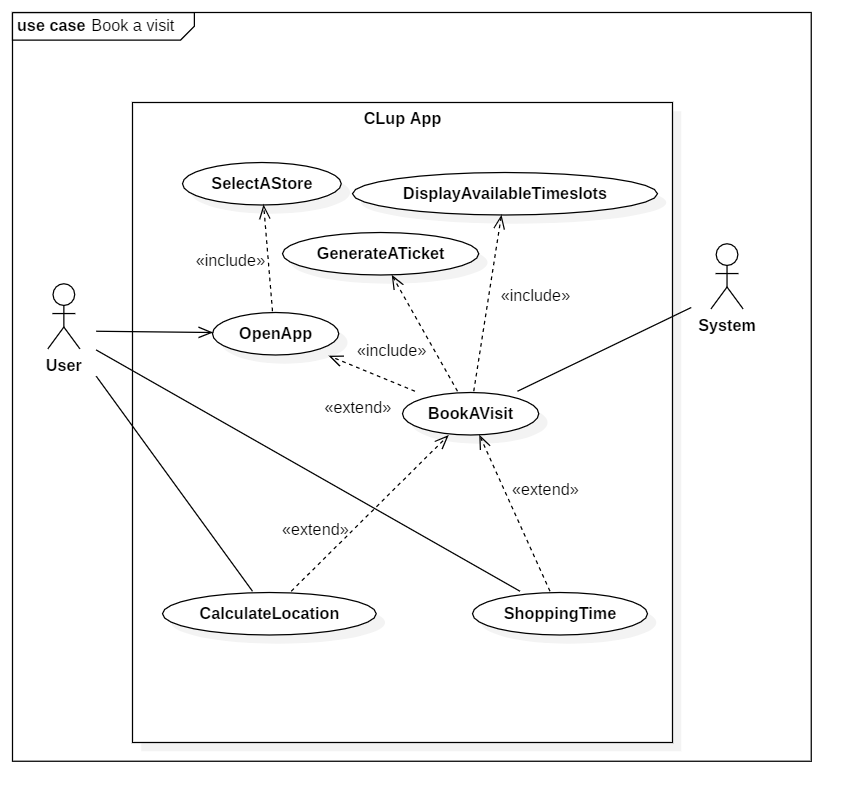
\includegraphics[width=\textwidth]{Images/UseCase1_BookAVisit}
\caption{\label{fig:usecase1}\textbf{Use case diagram 1 - Book a visit}}
\end{figure}

\begin{figure}[b]
\centering
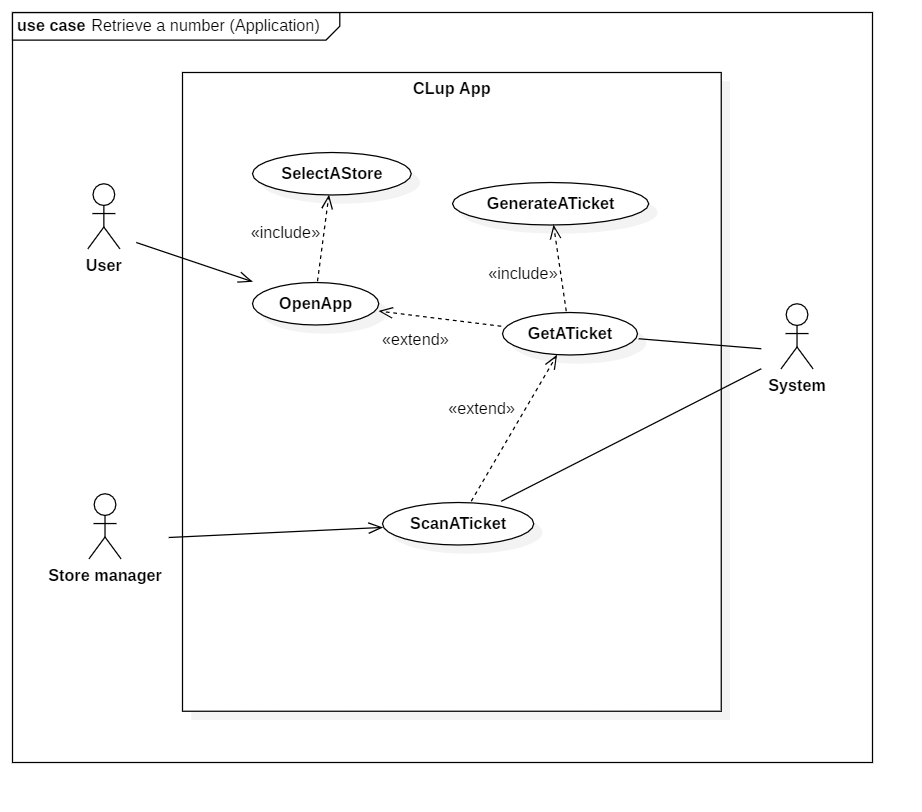
\includegraphics[width=\textwidth]{Images/UseCase2_RetrieveANumber}
\caption{\label{fig:usecase2}\textbf{Use case diagram 2 - Retrieve a number}}
\end{figure}

\pagebreak
\pagebreak
\newpage
\FloatBarrier
\subsubsection{Sequence diagrams}

\begin{figure}[!htb]
\centering
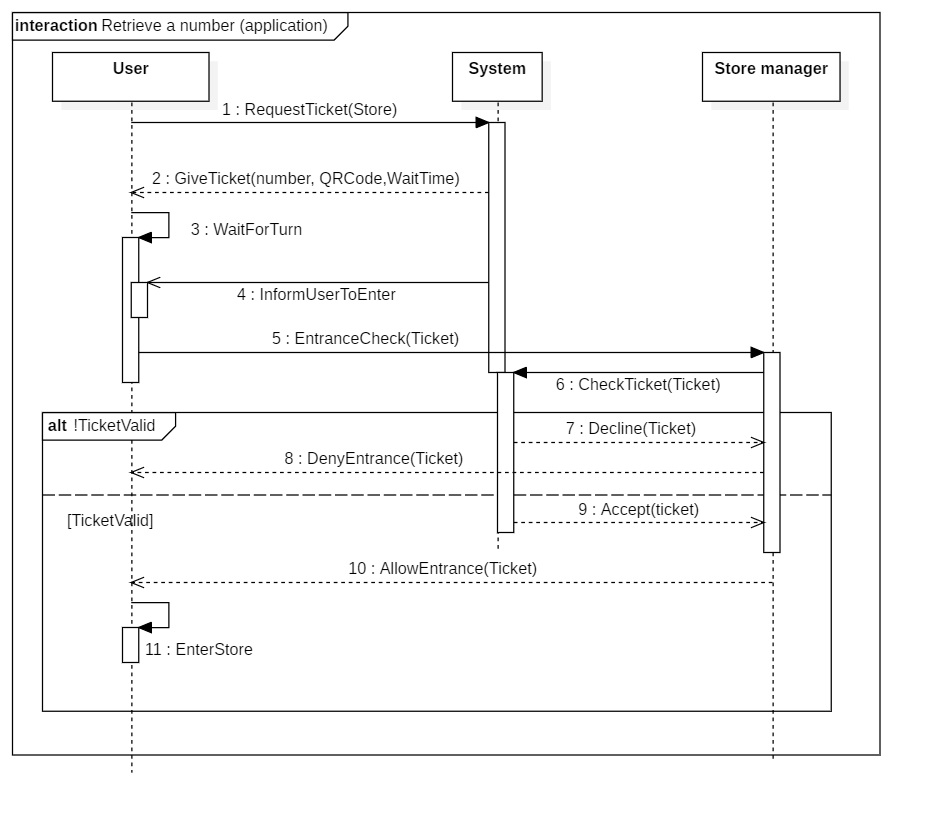
\includegraphics[width=\textwidth]{Images/SequenceDiagram1_RetrieveANumber}
\caption{\label{fig:sequence1}\textbf{Sequence diagram 1 - Retrieve a number}}
\end{figure}

\pagebreak

\begin{figure}[!htb]
\centering
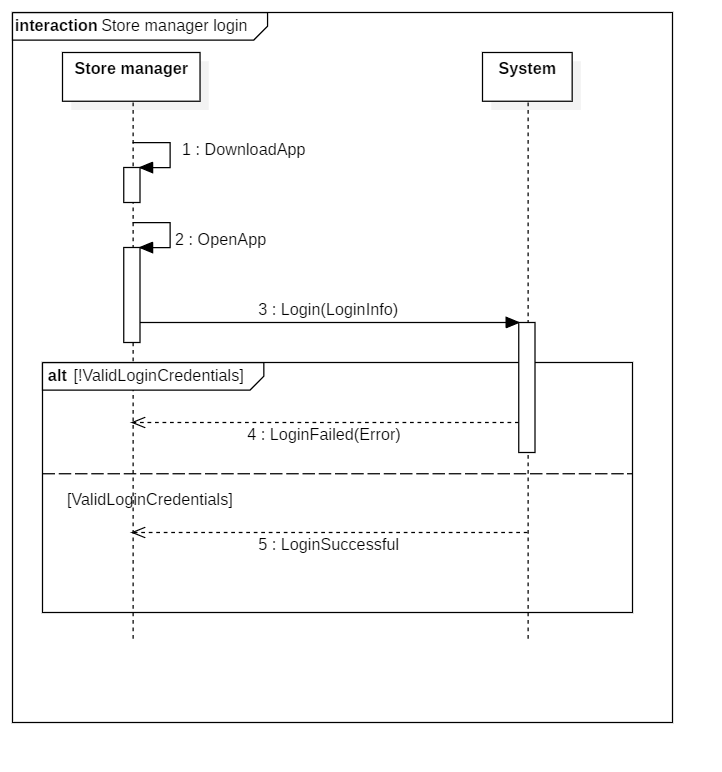
\includegraphics[width=\textwidth]{Images/SequenceDiagram2_StoreManagerLogin}
\caption{\label{fig:sequence2}\textbf{Sequence diagram 2 - Store manager login}}
\end{figure}

\pagebreak

\begin{figure}[!htb]
\centering
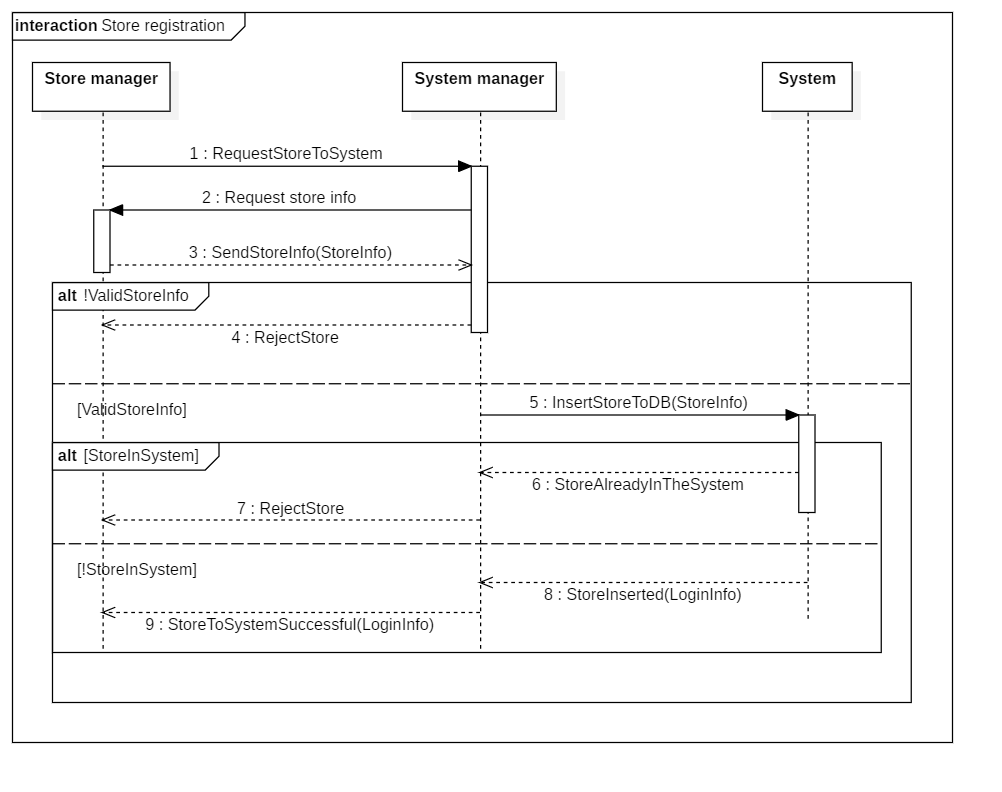
\includegraphics[width=\textwidth]{Images/SequenceDiagram3_StoreRegistration}
\caption{\label{fig:sequence3}\textbf{Sequence diagram 3 - Store registration}}
\end{figure}

\begin{figure}[b]
\centering
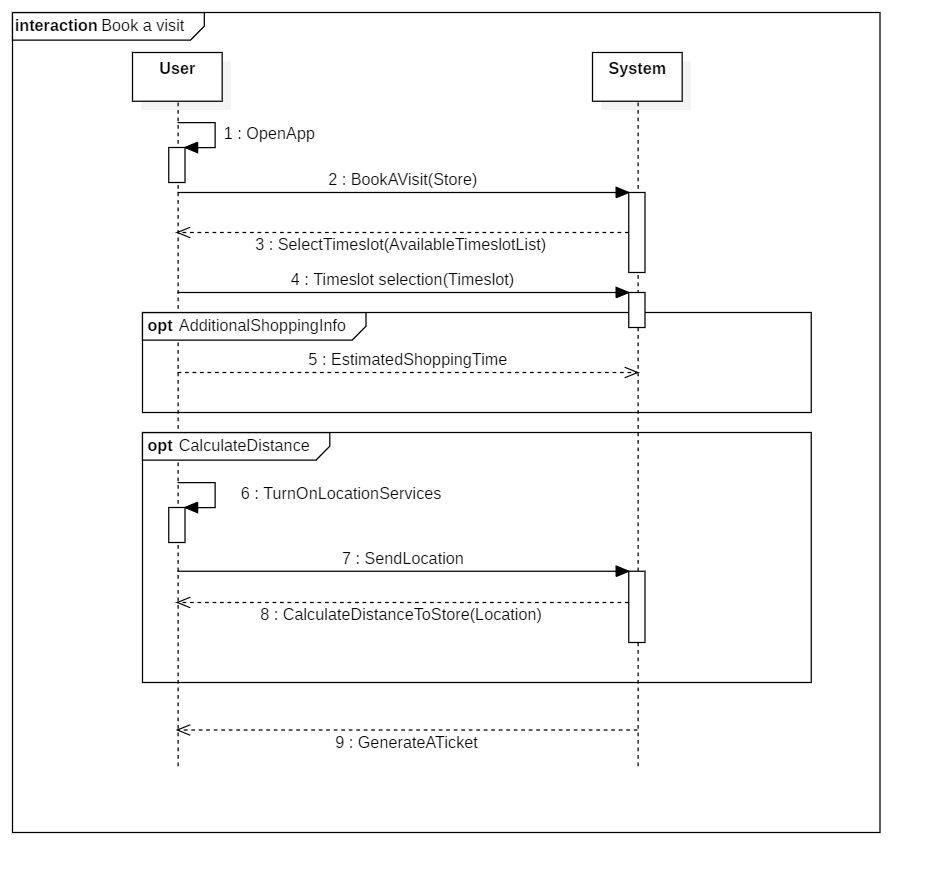
\includegraphics[width=\textwidth]{Images/SequenceDiagram4_BookAVisit}
\caption{\label{fig:sequence4}\textbf{Sequence diagram 4 - Book a visit}}
\end{figure}

\FloatBarrier
\newpage
\subsection{Performance requirements}

\hspace{\parindent}The system is relatively simple and doesn't work with a lot of data. What the system should do properly is control the queue for every specific store. It should also sync all of the tickets that are printed out in real life, and ones that are "printed" virtually. The same queue should feature both types of tickets and work adequately. That means that when a ticket is printed, it should be inserted into queue within ten seconds, to prevent errors in the queue. It is not of a major importance if a couple of people switch places due to slow reaction time from the system, but it should be avoided if possible. 


When user want to print a ticket virtually, the system has to provide it with an average waiting time within a couple of seconds. This is a piece of data that is going to be stored in the database of every store, and it should be updated at least every 30 minutes based on the current traffic and other available data, like day of the week and time of day.


When calculating the distance from the user's current location to the desired store, the information should be available to the user in ten seconds at most. If the system is for any reason unable to calculate the distance it should display a message that it it unable to do it and continue to the next step.

\newpage

\subsection{Design constraints}

\subsubsection{Standards compliance}
\hspace{\parindent}The entire application must be the subject to the General Data Protection Regulation (GDPR), a regulation in the EU law to protect the personal data of all individuals within the European Union (EU) and the European Economic Area (EEA).

\subsubsection{Hardware limitations} \label{hardware}

\hspace{\parindent}The application is only planned to be made for Android OS and iOS. Any device that doesn't use Android or iOS, but uses Windows Mobile OS is excluded from the use. Any non-smartphone mobile device will not support the application.

The application will only work on Android devices that support Android 5.0 (Lollipop) or above due to security reasons. 

The application will only work on iOS devices that support iOS 7.0 or above due to security reasons.

Device in use must have access to the internet connection during the ticket request. After it acquires the ticket, the internet connection is no longer required.
\subsubsection{Privacy limitations}

\hspace{\parindent} The application should not collect nor ask any personal information from the user. It should only request for access to publish push notifications, as well as location, but only if the user decides to use "Book a visit feature". No other data is to be collected at all. 

\newpage

\subsection{Software system attributes}
\subsubsection{Reliability and availability}
\hspace{\parindent}The system must be available at all times during the day. The only times that the system is allowed to be down, due to maintenance or any other reason, is during the night hours, while the stores are not working. In that time the use of application is nearly non-existent as only the "Book a visit" function is working, and the number of users using the function should be close to zero.

In case the system has stopped working during the day, a notification has to be sent to every user that uses the application, and the queueing in stores should be taken over by the store manager until the system is back up.

\subsubsection{Security}
\hspace{\parindent}Since there is no users' personal data that is stored within the system, the security by itself is at the very high level to begin with. Logins from the store managers should be encrypted and protected. Transfer of this data to the store managers should be done safely, either by using two-way encryption or in-person.

\subsubsection{Maintainability}
\hspace{\parindent}The system can be written in any language that will guarantee high level of maintainability and security at all times. It should also allow users to use the older version of the app, which means that every change made to the app must be made with legacy in mind. The code must have a clean and detailed documentation so that people who work on it have no problems upgrading the app and pushing new updates if necessary.

\subsubsection{Portability}
\hspace{\parindent}As already mentioned in the section \nameref{hardware}, the application should only work on Android and iOS mobile devices, with specific OS version limitations.

Application should not natively be supported with desktop devices since users must provide their QR code for scanning when entering the store, which would not be possible on a desktop computer, and not very usable on a laptop.
